\documentclass{article}
\usepackage[utf8]{inputenc}
\usepackage{fullpage}
\usepackage{verbatim}
\usepackage{graphicx}
\usepackage{float}

\title{RabbitMQ}
\author{Rohit Singh}
\date{June 19th - 25th, 2022}

\begin{document}

\maketitle

\tableofcontents

\section{Overview}

\subsection{What is RabbitMQ?}

RabbitMQ is a messaging broker which acts as an intermediary for messaging. RabbitMQ gives applications a common platform to send and receive messages, as well as a location to store messages until the are received.

\subsection{RabbitMQ Features}

\subsubsection{Reliability}

RabbitMQ allows applications to trade off performance with reliability. The reliability features that RabbitMQ allows for as persistence, delivery acknowledgements, publisher confirms and high availability.

\subsubsection{Flexible Routing}

RabbitMQ features built-in exchange types for typical routing logic. These exchanges can be combined together to create more complex routing mechanisms.

\subsubsection{Clustering}

Multiple RabbitMQ servers on a local network can be clustered together to form a single logical broker.

\subsubsection{Federation}
RabbitMQ offers a federation model to allow servers to be configured as loosely or unreliably as needed, even if clustered with other servers.

\subsubsection{Highly Available Queues}

RabbitMQ supports data structures like \textbf{replicated queues} and \textbf{streams}. With these structures, if there is a hardware failure, messages are safe as long as the majority of cluster nodes are online.

\subsubsection{Multi-Protocol}

RabbitMQ supports messaging over a variety of protocols, such as:

\begin{itemize}
    \item MQTT
    \item HTTP and WebSockets
    \item AMQP 1.0
\end{itemize}

\subsubsection{Software Clients}

There are RabbitMQ clients for almost any language that you can think of

\subsubsection{Management UI}

RabbitMQ ships with an easy-to use UI, allowing for simple monitoring and controlling of every aspect of the message broker.

\subsubsection{Tracing}

If the system is misbehaving, RabbitMQ offers tracing support for easier debugging.

\subsubsection{Plugin System}

RabbitMQ has numerous plugins that can be used to extend it in different ways. 
Custom plugins can also be created for more specific use cases.

\subsection{Dictionary}

\subsubsection{Producing}

\textbf{Producing} means nothing more than sending.

A program that sends messages is a \textbf{producer}

\subsubsection{Queue}

A \textbf{queue} is the name for a post box which lives inside RabbitMQ.

Although messages flow through RabbitMQ and applications, they are only stored in a \textit{queue}, which is bound by the host's memory and disk limits. 

Many \textit{producers} can send messages that go to one queue, and many \textit{consumers} can try to receive data from one \textit{queue}.

\subsubsection{Consuming}

\textit{Consuming} is the same as receiving. A \textit{consumer} is a program that mostly waits to receive messages.

\subsubsection{Message Acknowledgement}

\textit{Message Acknowledgement} lets us signal to the RabbitMQ server that a consumer has received and processed a given message. If RabbitMQ doesn't receive an acknowledgement, it means the consumer that was processing the node died or became disconnected, at which point the message is requeued and taken up by another worker.

\subsubsection{Message Durability}

\textit{Message Durability} ensures that the messages that are in the RabbitMQ server queue are not lost when the server goes offline. To ensure messages can survive server shutdowns, we need to make sure the queue they are sent to are durable and the message itself is durable, which is done via flags as shown in section \textit{2.2 Work Queues}

\subsubsection{Exchanges}

\textit{Exchanges} are exactly what they sound like, a construct that takes messages and exchanges it to the queue. In reality, clients don't publish directly to queues, instead they hand the message to an exchange, which knows exactly what to do with the message based on a set of rules defined in the \textit{exchange type}

\section{Tutorials}

\subsection{Note on RabidsMQ}

After the 2nd tutorial, I realized the amount of reused code and saw the need for a resuable class to make life more easy. Because of this, a lot of the code talked about in the first two tutorials have been refactored and placed in the \verb|RabidsMQ| class located \verb|RabbitMQ/RabidsMQ.py|.

This class is just a simple manager for RabbitMQ clients, and the explanations behind the code in the first two tutorials still applies, only located in a different file.

\subsection{Hello World!}

\textit{Source code located at}: \verb|the-big-repository-of-knowledge/RabbitMQ/tutorials/hello_world/|

\subsubsection{Introduction}

In this example, we are writing two programs in Python programs, one to act as the producer and another to act as a consumer. The producer will send a single message to the consumer which will print it out upon receiving it. 

The overall design will look like: 

\begin{figure}[H]
    \centering
    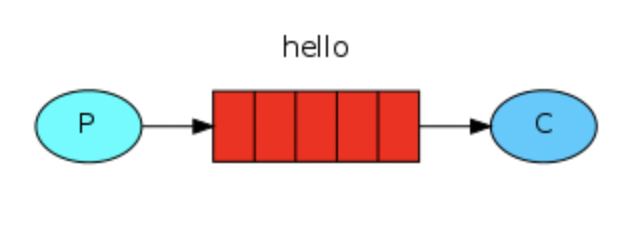
\includegraphics[scale=0.8]{RabbitMQ/images/t1-1.png}
    \caption{System Diagram (from https://www.rabbitmq.com/tutorials/tutorial-one-python.html)}
    \label{t1-1}
\end{figure}

\subsubsection{Producer}

The first thing we need to do when we are creating a sender is understand where we are sending the message to. For this example, we use \verb|localhost|, and we connect with:

\begin{verbatim}
    o_ConnectionParameters = pika.connectionParameters('localhost')
    o_Connection = pika.BlockingConnection(o_ConnectionParameters)
\end{verbatim}

We create a \verb|BlockingConnection| to ensure the rest of the program doesn't continue until we have successfully connected to the target specified by \verb|o_ConnectionParameters|.

Once \verb|o_Connection| has been successfully created, we need to open a channel on the connection, which we do with:

\begin{verbatim}
    o_Channel = o_Connection.channel()
\end{verbatim}

Now that the communication channel is created, we need to declare a queue to which the message will be published. As shown in the diagram above, we name the queue "hello":

\begin{verbatim}
    o_Channel.queue_declare("hello")
\end{verbatim}

Once the queue has been successfully declared, we can finally send a message! To send a message, we do:

\begin{verbatim}
    o_Channel.basic_publish(
        exchange    = '',
        routing_key = 'hello',
        body        = 'Hello, World!"
    )
\end{verbatim}

From this, we can see that \verb|o_Channel.basic_publish| has 3 parameters that we are using here:

\begin{itemize}
    \item \verb|exchange|: All messages need to go through an exchange before entering the queue. This is discussed more in tutorial 3
    \item \verb|routing_key|: Specifies the queue name
    \item \verb|body|: Contains the body of the message being sent.
\end{itemize}

After we have sent the message, we close the connection to be thorough, which can be done with:

\begin{verbatim}
    o_Connection.close()
\end{verbatim}

We need to ensure that RabbitMQ is running, for which we just use the pre-built Docker image:

\begin{verbatim}
    docker run -it --rm --name rabbitmq -p 5672:5672 -p 15672:15672 rabbitmq:3.10-management
\end{verbatim}

Once this is up and running, we run the program to send the message, which pushes it into the queue.

\subsubsection{Consumer}

Here, like we did with the producer, we create a connection to localhost using the same code.

Once the connection is created, we connect to the same queue with the same code used before. Although the previous time running the \verb|queue_declare| code created the queue, running it again will not create a new one, but connect to the existing one.

Beyond these similarities, creating a consumer is more involved than creating a publisher. 

The first step to creating a consumer is defining a function that will handle message receives:

\begin{verbatim}
    def callback(ch, method, properties, body):
        print(f"[<----] Received {body}")
\end{verbatim}

Once we define the function, we need to attach it to the queue, which we do with:

\begin{verbatim}
    o_Channel.basic_consume(
        queue='hello',
        auto_ack=True,
        on_message_callback=callback
    )
\end{verbatim}

This function is provided the following values:

\begin{itemize}
    \item \verb|queue|: Defines the queue to attach to
    \item \verb|auto_ack|: Explained later
    \item \verb|on_message_callback|: Attaches callback function to queue
\end{itemize}

Once we have told the queue what how to consume messages, we need to tell it to start consuming:

\begin{verbatim}
    o_Channel.start_consuming()
\end{verbatim}

For good measure, we wrap the code in a \verb|KeyboardInterrupt| clause to allow for graceful shutdown, as shown in the source code.

\subsection{Task / Work Queues}

\textit{Source code located at}: \verb|the-big-repository-of-knowledge/RabbitMQ/tutorials/task_queue/|

\subsubsection{Introduction}

The motivation for task queues is to allow us to avoid doing a resource-intensive task immediately and having to wait for it to complete. Instead, we schedule the task to be done later.

To schedule the task, we first need to encapsulate it into a message and send it to the queue, and eventually a worker process in the background will pop messages off the queue and execute the job. When there are multiple running workers, the task is split between them.

This concept is especially useful in applications like web apps, where it's impossible to handle a complex task in the short HTTP request window.

In tutorial 1, we sent a simple message containing \textit{Hello, World!} to the queue. In this tutorial, we will be sending strings that represent tasks. 

When we send a message from our producer, it will be placed in the queue where it remains until consumed by the consumer, at which point \verb|time.sleep()| is triggered to simulate a resource heavy task, with the sleep time determined by the number of dots at the end of the message.

One advantage of using task queues is \textbf{round robin dispatching}. This is a process by which we parallelize work loads. If we have a backlog of work, we can add more consumer replicas to tackle the backlog.

Note that round robin dispatching does not assign tasks by the current workload a worker is given, instead just always assigning backlogged tasks to the next node. This means that when if we have two nodes, A and B, and node A is executing a large task, if two small tasks will come in, one will be sent to B and the other sent to A. This isn't ideal, since we would prefer if the non-working node B, handles the two small tasks while A is still working on the large task.

\subsubsection{Producer}

This program will allow us to read the commandline to send messages, so we add the following line of code to define our message:

\begin{verbatim}
    s_Message = ' '.join(sys.argv[1:]) or "Default Message"
\end{verbatim}

We also need to define a function to initialize the channel, which is done the same way as in tutorial 1:

\begin{verbatim}
    def openChannel(s_Host='localhost'):
        # Open Connection Channel
        o_ConnectionParameters = pika.ConnectionParameters(s_Host)
        o_Connection    = pika.BlockingConnection(o_ConnectionParameters)
        o_Channel       = o_Connection.channel()
        return o_Channel
\end{verbatim}

We create another queue to communicate our messages to, and send the message:

\begin{verbatim}
    # Declare message queue
    o_Channel.queue_declare(queue='tutorial_2')
    # Send the message
    o_Channel.basic_publish(
        exchange='',
        routing_key='tutorial_2',
        body=s_Message)
\end{verbatim}

\subsubsection{Consumer}

The consumer here is largely the same as the consumer outlined in tutorial 1. In the source code, the major differences are just from refactoring and the new consumer callback function:

\begin{verbatim}
    def callback(ch, method, properties, body):
        print(f"[<----] Received {str(body)}")
        time.sleep(body.count(b'.'))
        print("[X] Done")
        ch.basic_ack(delivery_tag = method.delivery_tag)
\end{verbatim}

\subsubsection{Message Acknowledgement}

The new \verb|ch.basic_ack| line is used to send message acknowledgements back to the RabbitMQ server. As explained in the \textit{Dictionary} section, \textit{message acknowledgements} ensure if the consumer currently working on a message disconnects, the message will be requeued by the server and taken up by another consumer.

\subsubsection{Message Durability}

We want to make sure our messages are durable, that is, that they will survive the RabbitMQ server going offline. To do this, we need to change the \verb|o_Channel.queue_declare(queue='tutorial_2')| and \verb|o_Channel.basic_publish(exchange='',routing_key='tutorial_2',body=s_Message)| to:

In both consumer and producer files:

\begin{verbatim}
    o_Channel.queue_declare(queue='task_queue', durable=True)
    
    o_Channel.basic_consume(
        queue                   = 'task_queue',
        on_message_callback     = callback
    )
\end{verbatim}


In just the producer file:

\begin{verbatim}
    o_Channel.basic_publish(exchange='',
        routing_key="task_queue",
        body=s_Message,
        properties=pika.BasicProperties(
            delivery_mode = pika.spec.PERSISTENT_DELIVERY_MODE
        )
    )
\end{verbatim}

\subsubsection{Fair Dispatch}

Like mentioned earlier, round robin dispatching doesn't allow for fair distribution across nodes. We can specify fair dispatching by adding the following property to our \verb|o_Channel| in our consumer file.

\begin{verbatim}
    o_Channel.basic_qos(prefetch_count=1)
\end{verbatim}

This tells RabbitMQ not to give more than 1 message to a worker at a time. This ensures that if a worker is still processing a task, check if there are empty workers that can take the backlogged task instead.

\subsubsection{Conclusion}

Here we have shown how we can use RabbitMQ to define task queues to allow for load balancing across worker nodes for resource heavy tasks, as well as how to ensure that our messages are durable and there are contingencies in place to resolve the message in case a worker or RabbitMQ server dies unexpectedly.

\subsection{Publish/Subscribe}

\textit{Source code located at}: \verb|the-big-repository-of-knowledge/RabbitMQ/tutorials/publish_subscribe/|

\subsubsection{Introduction}

When we discussed work queues, we were operating under the assumption that every task is only being distributed to a single consumer. What if we wanted to deliver messages to multiple consumers? That is what we will do now.

We are going to create two programs, \verb|log_emitter.py| and \verb|log_consumer.py|. The former will create logs and the latter will consume and print them.

In previous tutorials, we used empty exchanges which allowed producers to queues, which we don't want. Instead, we want producers to send messages to an \textbf{exchange}. 

From dictionary:

\textit{Exchanges} are exactly what they sound like, a construct that takes messages and exchanges it to the queue. In reality, clients don't publish directly to queues, instead they hand the message to an exchange, which knows exactly what to do with the message based on a set of rules defined in the \textit{exchange type}

Although there are many types of exchanges, we are going to use \verb|fanout|. 

\subsubsection{Log Emitter}

To get started, we add the following to \verb|log_emitter.py|

\begin{verbatim}
    # Define RabidsMQ instance
    o_Rabids = RabidsMQ(s_Host='localhost')
    # Open channel
    o_Rabids.openChannel()
    # Declare the exchange
    o_Rabids.o_Channel.exchange_declare(
        exchange='logs',
        exchange_type='fanout'
    )
\end{verbatim}

The main difference between this and the rest of the tutorials is that we now invoke the \verb|.exchange_declare()| to specify where to send the messages and what type of exchange to use.

We wrap up the \verb|log_emitter.py| the same way we wrapper up our other \verb|producers|

\begin{verbatim}
    # Create message
    s_Message = ' '.join(sys.argv[1:]) or "Default Log"
    # Publish to the exchange
    o_Rabids.basicPublish(
        s_Exchange      = 'logs',
        s_RoutingKey    = '',
        s_Body          = s_Message
    )
    # Close the queue
    o_Rabids.o_Channel.close()
\end{verbatim}

It is worth noting that now we do not specify the \verb|s_RoutingKey|, since the producer doesn't know what queue the message is going to, instead it only knows that it is going to the exchange that we declared in the channel.

\subsubsection{Log Consumer}

Rather than telling our consumer to listen to a specific queue as we have done before, we are now using \textbf{temporary queues}. This is because we want our consumer to listen to all log messages, not just a subset of them. To ensure this, we create our consumer as follows:

\begin{verbatim}
    # Define Rabids MQ instance
    o_Rabids = RabidsMQ(s_Host='localhost')
    # Open channel 
    o_Rabids.openChannel()
    # Declare exchange
    o_Rabids.o_Channel.exchange_declare(exchange='logs', exchange_type='fanout')
    # Store the resulting queue name
    s_QueueName = o_Rabids.o_Channel.queue_declare(queue='', exclusive=True).method.queue
    # Bind the channel's queue to the exchange
    o_Rabids.o_Channel.queue_bind(exchange='logs', queue=s_QueueName)
    print("Waiting for logs...")
    o_Rabids.basicConsume(
        s_Queue=s_QueueName,
        F_Callback= lambda x: x = x,
        b_AutoAck=True
    )
    # Start consuming
    o_Rabids.o_Channel.start_consuming()
\end{verbatim}

Notice that now, instead of binding the consumer directly to a queue, it is attached to an exchange and then after we declare the exchange we instead allow the queue to be declared randomly (by giving queue declare a blank queue) which we then bind to the exchange.

Now, we can open two log consumers, and pipe one to an output file to both see the logs from one consumer and save them with another.

\subsubsection{Conclusion}

Here we have shown the value of exchanges, changed our approach to not publish directly to queues. and ensure that we can send messages to multiple consumers at the same time.

\subsection{Routing}

\textit{Source code located at}: \verb|the-big-repository-of-knowledge/RabbitMQ/tutorials/routing/|

\subsubsection{Introduction}

Last tutorial, we created a logging system that could broadcast messages from a single client to many receivers via exchanges rather than queues. 

The problem with the system implemented in the last tutorial is that every subscribed client received every message published to the exchange. Imagine if over a distributed system every client received every message published, it would be a mess! 

Now, we are going to add functionality so that clients can subscribe to only receive a subset of the messages.

The files in this section are largely the same as the files in \textit{tutorial 3: Publish / Subscribe}, so we will focus more on the difference between the two files, with the complete source code for this file located in the GitHub repository.

\subsubsection{Bindings}

In the last section, we used bindings to connect an exchange to a queue, but we omitted a \verb|routing_key| parameter. This parameter can be used to specify the \textit{topic} of messages being routed through the exchange to the queue.

For example:

\begin{verbatim}
    o_Rabids.o_Channel.queue_bind(
        exchange    = "Basic Exchange",
        queue       = "Basic Queue",
        routing_key = "Logs"
    )
\end{verbatim}

This code will bind the exchange "Basic Exchange" to the queue "Basic Queue", and it will \textit{basically} tag all messages sent from Basic Exchange to Basic Queue as "Logs". This way, the clients that are interested in logs can handle them as they wish, and ones that are not interested can ignore them completely.

\subsubsection{Direct Exchange}

Now that we can tag messages with a topic, we want to be able to filter messages based on their tags. 

To fix this, we need to change our exchange type, since we were previously using \verb|fanout|, which is only capable of mindless broadcasting from an exchange to multiple queues.

We could instead use a \verb|direct| exchange which forwards messages with a routing key that matches that of the queues binding key.

It is important to note that we can have more than one routing key attached to a queue's binding key, that is, queues can have multiple bindings.

Even further, exchanges can bind multiple routing keys to different queues, that is, two queues can receive messages of the same topics.

\subsubsection{Log Emitter}

The main differences in this log emitter and the one from tutorial 3 can be seen below:

\begin{verbatim}
    s_Severity = ' '.join(sys.argv[2]) or "LOW"
    # Declare the exchange
    o_Rabids.o_Channel.exchange_declare(
        exchange='direct_logs', 
        exchange_type='direct' =
    )
    # Publish to the exchange
    o_Rabids.basicPublish(
        s_Exchange      = 'direct_logs',
        s_RoutingKey    = s_Severity,
        s_Body          = s_Message
    )
\end{verbatim}

Notice that we are now defining a routing key from the command line arguments, and sending the messages depending on the provided argument.

\subsubsection{Log Consumer}


The main differences between this file and the previous \verb|log_consumer| from tutorial 3 can be seen below:

\begin{verbatim}
    o_Rabids.o_Channel.exchange_declare(exchange='direct_logs', exchange_type='direct')
    # Store the resulting queue name
    s_QueueName = o_Rabids.o_Channel.queue_declare(queue='', exclusive=True).method.queue
    # Bind the channel's queue to the exchange depending on severites
    a_Severities = sys.argv[1:]
    for s_Severity in a_Severities:
        o_Rabids.o_Channel.queue_bind(exchange='direct_logs', queue=s_QueueName, routing_key=s_Severity)
\end{verbatim}

Like we parsed the severity of the message in the log emitter, here we are specifying the topic that the client is listening for. Depending on the severity we provide the client, we bind the queue to each severity. Note this part is very similar to the last tutorial, with the main difference being that we perform multiple queue binds.

\subsubsection{Conclusion}

We can demo this by opening 3 programs, one producer and 2 consumers. The consumers should be specified with \verb|python3 log_consumer.py HIGH| and \verb|python3 log_consumer.py LOW MED|. Now, we can run producers with \verb|python3 log_emitter {LOG_MESSAGE} {SEVERITY}|. If we specify severity to be \verb|LOW| or \verb|MED|, it will go to the second consumer, and if we specify it to be \verb|HIGH|, it will go to the first. Any other severities will not be processed by the consumer nodes. 

Here we have learned how to filter and route messages depending on their topics, and how this can be used to ensure only interested clients receive important messages they care about.

\subsection{Topics}

\textit{Source code located at}: \verb|the-big-repository-of-knowledge/RabbitMQ/tutorials/topics/|

\subsubsection{Introduction}

Last tutorial, we used a direct exchange to allow for routing and filtering based on topics. This still has some limitations, mainly that \verb|direct| only allows for a message to have a single topic. This is not ideal, as we often want to route messages to a specific client based on multiple criteria.

\subsubsection{Topic Exchange}

Instead of using a \verb|fanout| or \verb|direct| exchange, we are going to use a \verb|topic| exchange.

Messages sent to a topic exchange must not have arbitrary routing keys, but instead a list of word delimited by dots: \verb|car.sensors.imu.acceleration.lateral|.

The binding key of a queue must be in the same form, so a client that wants all car data will subscribe to a queue with binding key \verb|car.#|, and another client that just wants acceleration data will subscribe to a queue with binding key \verb|car.sensors.imu.acceleration.*|

In this example, we are going to send messages that describe F1 car telemetry. There are two queues with 3 bindings:

\begin{itemize}
    \item Queue 1 is interested in engine health (\verb|car.engine.#|)
    \item Queue 2 is interested in tyre degradation and hydraulics (\verb|car.tyre.*.degradation| and \verb|car.hydraulics.#|)
\end{itemize}

Once again, the code here is quite similar to the previous tutorial, so we will focus on the discussion of the differences only.

\subsubsection{Data Emitter}

The main differences between this data emitter and the log emitter from the last tutorial can be seen below:

\begin{verbatim}
    s_Message   = (sys.argv[1]) or "Empty Data"
    s_Topic     = (sys.argv[2]) or "anonymous.data"
    # Declare the exchange
    o_Rabids.o_Channel.exchange_declare(
        exchange='topic_logs', 
        exchange_type='topic'
    )
    # Publish to the exchange
    o_Rabids.basicPublish(
        s_Exchange      = 'topic_logs',
        s_RoutingKey    = s_Topic,
        s_Body          = s_Message
    )
\end{verbatim}

Notice that all we have done different is change the exchange name and the type, and assign a more complex routing key to the publish function than earlier.

\subsubsection{Data consumer}

The main differences between this consumer and the consumer from the last tutorial can be seen below:

\begin{verbatim}
    o_Rabids.o_Channel.exchange_declare(exchange='topic_logs', exchange_type='topic')
    # Store the resulting queue name
    s_QueueName = o_Rabids.o_Channel.queue_declare(queue='', exclusive=True).method.queue
    # Bind the channel's queue to the exchange depending on severites
    a_Topics = sys.argv[1:]
    for s_Topic in a_Topics:
        o_Rabids.o_Channel.queue_bind(exchange='topic_logs', queue=s_QueueName, routing_key=s_Topic)
    # Wait for logs
\end{verbatim}

Similarly to the emitter, all we do is change the routing keys to more complex topics and change the exchange declare.

\subsubsection{Conclusion}

Now we can test our system by running 3 programs. One producer publishing to different topics from the command line. For example: 

\verb|python3 data_emitter.py 5% car.tyres.1.degradation|

or 

\verb|python3 data_emitter.py GOOD car.engine.ICE)|

Then we can start two consumers:

\verb|python3 data_consumer.py "car.tyres.*.degradation" "car.hydraulics.#"|

and

\verb|python3 data_consumer.py "car.engine.#"|

Whenever we trigger our emitters, depending on the topic we declare to each message we will see the message sent to only the client interested, even if we fill the wildcards (* and \#) with whatever we want.

Here we have seen how to create more complex topics as routing keys to allow for more refined routing and filtering.

\end{document}